\chapter{\babEmpat}
Di bab ini, diberikan petunjuk penggunaan khusus ditujukan bagi responden, khususnya ketika responden belum dapat menyelesaikan penilaian diri dan harus melanjutkannya di waktu yang akan datang. Diharapkan para pengelola satker dapat memberikan penjelasan jika ada pertanyaan. \figurename~\ref{fig:jeda} memberikan ilustrasi bahwa responden telah menyelesaikan beberapa penilaian.

\begin{figure}
  \begin{center}
    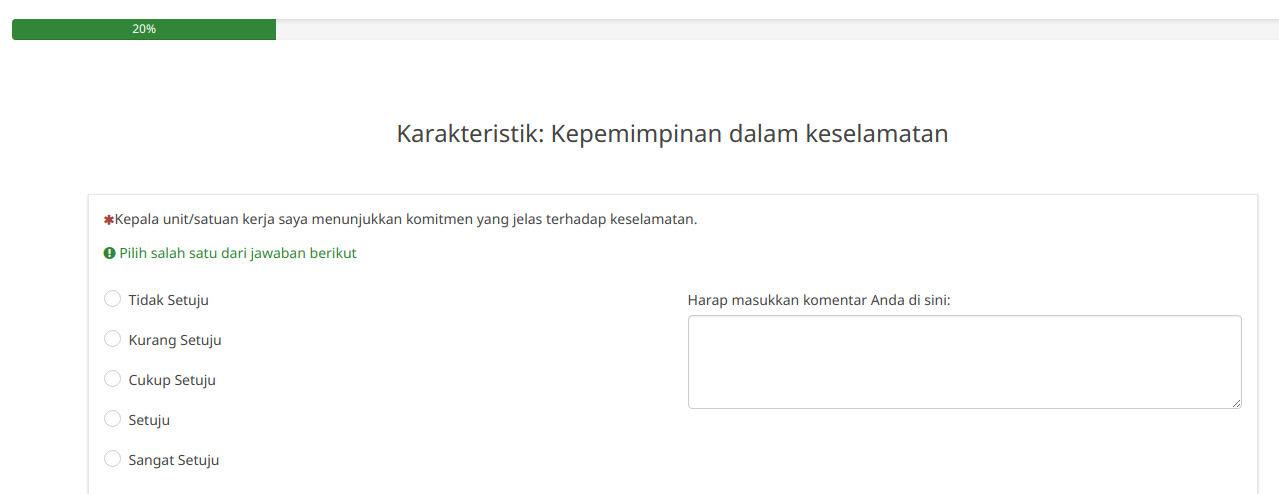
\includegraphics[scale=.35]{pics/masukLagi2.png}
    \caption{Responden telah sampai pada pada kelompok pertanyaan kedua}
    \label{fig:jeda}
  \end{center}
\end{figure}
 
Jika di posisi seperti \figurename~\ref{fig:jeda} reponden ingin berhenti dan melanjutkan lagi lain waktu, responden harus melakukan klik pada tombol \texttt{Lanjutkan nanti} seperti diilustrasikan pada \figurename~\ref{fig:jeda}.

\begin{figure}
  \begin{center}
    
\includegraphics[scale=.5]{pics/masukLagi0.png}
    \caption{Responden melanjutkan penilaian diri lain waktu}
    \label{fig:jeda}
  \end{center}
\end{figure}
 
 
Selanjutnya, responden akan menjumpai dialog seperti \figurename~\ref{fig:lanjutLagi}. Terlihat bahwa informasi surat elektronik tidak diwajibkan. Sehingga identifikasi penilaian diri menggunakan parameter \texttt{Nama}. Bahkan jika parameter \texttt{Nama} sudah pernah digunakan oleh responden lain, akan muncul peringatan seperti \figurename~\ref{fig:lanjutLagi1}.

\begin{figure}
  \begin{center}
    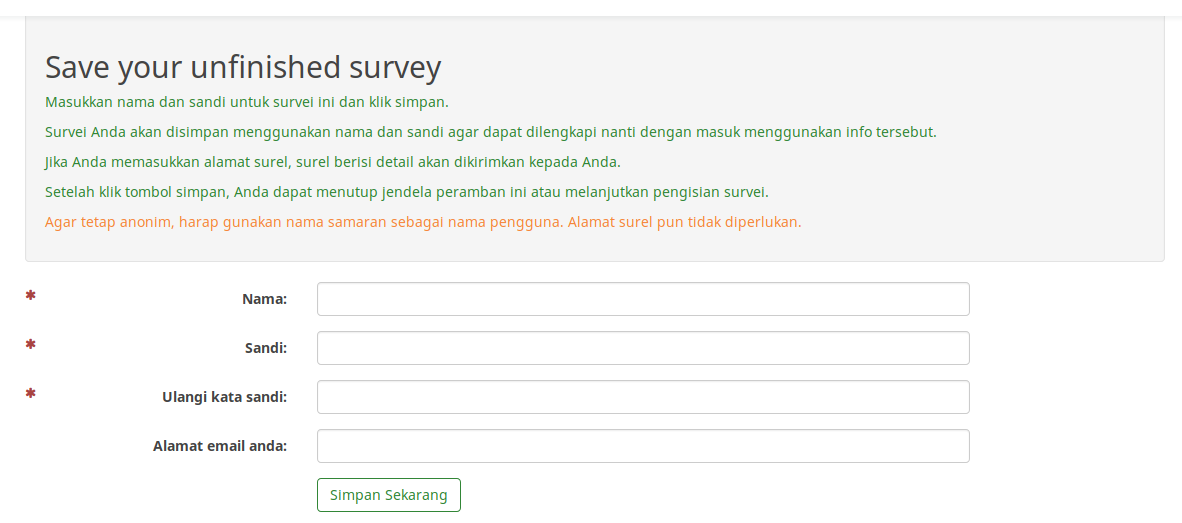
\includegraphics[scale=.35]{pics/lanjutLagi.png}
    \caption{Informasi yang diperlukan untuk melanjutkan penilaian diri}
    \label{fig:lanjutLagi}
  \end{center}
\end{figure}

\begin{figure}
  \begin{center}
    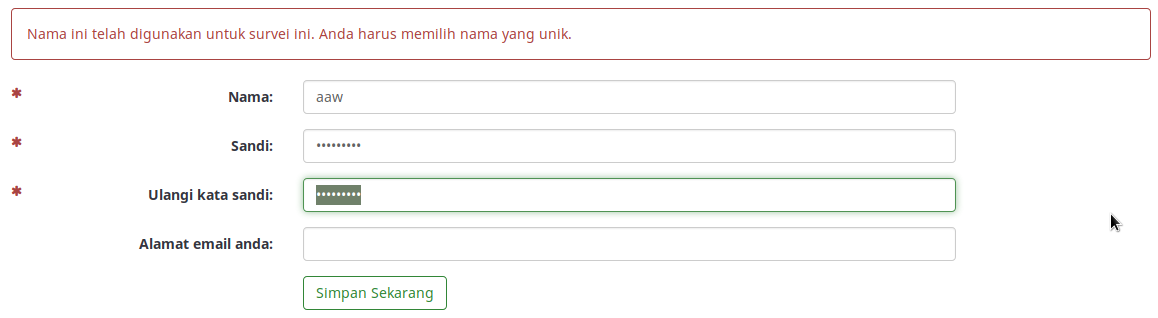
\includegraphics[scale=.5]{pics/lanjutLagi1.png}
    \caption{Parameter \texttt{Nama} telah digunakan}
    \label{fig:lanjutLagi1}
  \end{center}
\end{figure}

Jika informasi yang diminta telah dimasukkan, maka responden akan menjumpai dialog konfirmasi seperti \figurename~\ref{fig:surveyDisimpan} berikut. Konfirmasi tersebut akan dimunculkan setiap responden selesai melakukan penilaian diri, apakah selesai sebagian maupun keseluruhan. Jika selesai sebagian, halaman penilaian diri selanjutnya menjadi tidak aktif seperti diilustrasikan \figurename~\ref{fig:gakBsLanjut}.

\begin{figure}
   \begin{center}
     
\includegraphics[scale=.5]{pics/surveyDisimpan.png}
     \caption{Konfirmasi penilaian diri telah disimpan}
     \label{fig:surveyDisimpan}
   \end{center}
 \end{figure} 
 
\begin{figure}
   \begin{center}
     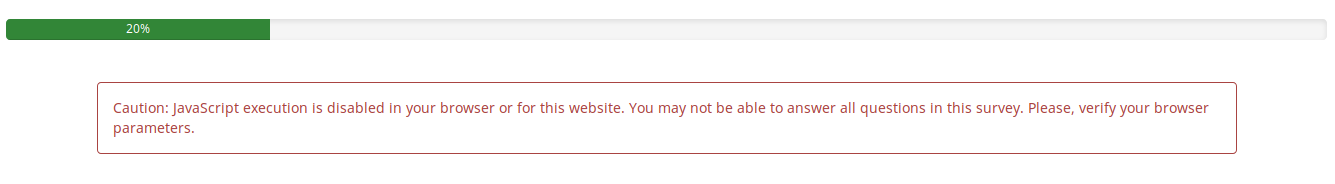
\includegraphics[scale=.35]{pics/gakBsLanjut.png}
     \caption{Penilaian diri untuk sementara tidak bisa dilanjutkan karena responden belum dapat melanjutkannya saat ini}
     \label{fig:gakBsLanjut}
   \end{center}
 \end{figure}
